\documentclass{standalone}
\usepackage{tikz,color}
\usetikzlibrary{decorations.pathreplacing}

\begin{document}
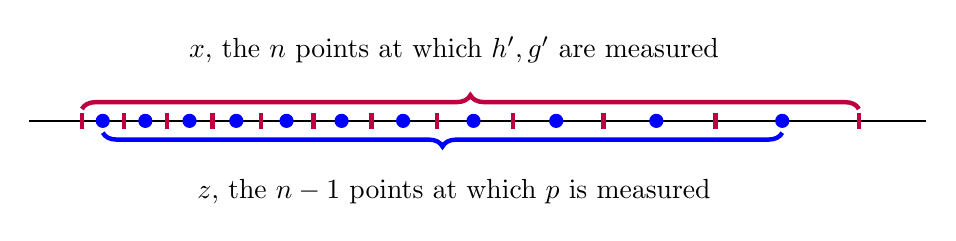
\begin{tikzpicture}[scale=1.5]

\draw  [thick] (-0.1,0) to (7.5,0);

\draw [blue, ultra thick,decorate, decoration={brace,mirror,amplitude=5pt}]
({4*tan(7.5)},-0.1) -- ( {4*tan(57.5)}, -0.1);

\draw [purple, ultra thick, decorate, decoration={brace,amplitude=5pt}]
({4*tan(5)},0.1) -- ( {4*tan(60)}, 0.1);

\foreach \x in {1,...,12}
   \draw [ultra thick, purple] ({4*tan(\x*5)},-0.07) -- ({4*tan(\x*5)},0.07);

\foreach \x in {1,...,11}
   \fill [blue] ({4*tan(\x*5+2.5)},0) circle [radius=0.06];

\node at (3.5,0.6) {$x$, the $n$ points at which $h',g'$ are measured};
\node at (3.5,-0.6) {$z$, the $n-1$ points at which $p$ is measured };

\end{tikzpicture}
\end{document}
